\documentclass{beamer}
\usetheme{tumkdd} %  TUM KDD beamer theme (beamerthemetumkdd.sty)

\usepackage{graphicx}
\usepackage{pgfplots}         % Plots in Latex
\usepackage{amsmath, amssymb} % Math formulas and symbols
\usepackage{tikz}
\usetikzlibrary{arrows,shapes}

\title[Passing and propagation]{Message passing and expectation propagation}
%\subtitle{Presentation subtitle}
\date{29 May 2017}
\author{Christoph Dehner}
\institute[TUM]
{Technische Universit\"at M\"unchen\\
Department of Informatics\\
Data Mining and Analytics\\
\textcolor{tum}{\url{kdd.in.tum.de}}\\
}

\begin{document}
\begin{frame}
    \titlepage
    \thispagestyle{empty}
\end{frame}

\begin{frame}{Overview}
	Graphical models: Bayesian networks and Markov random fields\\
	\begin{equation*}
	p(X)= \prod_{s} f_s(X_s)
	\end{equation*}
	
	Inference in graphical models:\\
	\begin{itemize}
		\item Marginalization
		\item Maximum aposteriori estimation
		\item Posterior approximation
	\end{itemize}
	

\end{frame}

\begin{frame}{Motivation for marginalization}
	
	
	\begin{figure}
		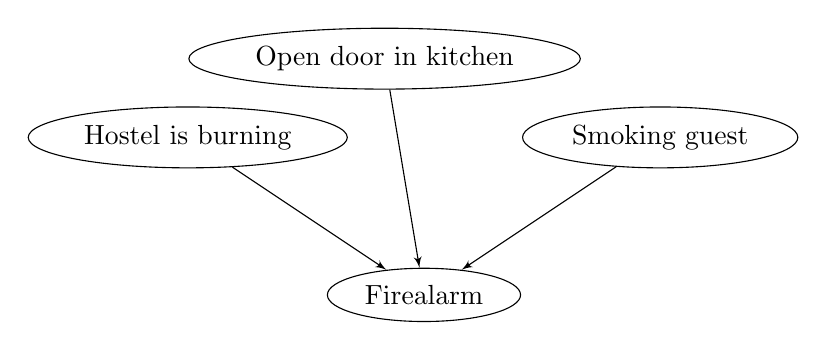
\begin{tikzpicture}
		
		\tikzset{vertex/.style = {shape=ellipse,draw,minimum size=1.5em}}
		\tikzset{edge/.style = {->,> = latex'}}
		
		\node[vertex] (x1) at  (3,-2) {Smoking guest};
		\node[vertex] (x2) at  (-3,-2) {Hostel is burning};
		\node[vertex] (x3) at  (0,-4) {Firealarm};
		\node[vertex] (x4) at  (-0.5,-1) {Open door in kitchen};
		%\node[vertex] (x5) at  (-0.5,1) {Breakfast is prepared};
		
		\draw[edge] (x1) to (x3);
		\draw[edge] (x2) to (x3);
		\draw[edge] (x4) to (x3);
		%\draw[edge] (x5) to (x4);
		\end{tikzpicture}
	\end{figure}
	%\centering
	%\begin{columns}[c] % the "c" option specifies center vertical alignment
%		\column{.5\textwidth} 
%		\only<2->{\includegraphics[scale=0.25]{BN_example.png}}
%		\column{.5\textwidth} 
%		\only<3->{\includegraphics[scale=0.25]{MRF_example.jpg}} 
%	\end{columns}
%	
%	\raggedright
%	\tiny{\only<2->{Image sources:\\
%%ttp://www.bayesia.com/hs-fs/hubfs/Bayesian\_Networks/Fig\_2\_2\_Sprinkler.png?t=1495201256220\\\&width=450\&height=626\&name=Fig\_2\_2\_Sprinkler.png\\}
%	\only<3->{http://homepages.inf.ed.ac.uk/rbf/CVonline/LOCAL\_COPIES/AV0809/ORCHARD/mrf.jpg}}
\end{frame}

\begin{frame}[t]{Factor graph}
	More simple and formally:\\
	\centering
	$p(X) =  p(x_1) p(x_2|x_1) p(x_3|x_1)$\\
	\begin{figure}
		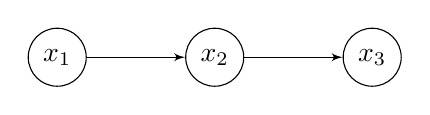
\begin{tikzpicture}
		
		\tikzset{vertex/.style = {shape=circle,draw,minimum size=1.5em}}
		\tikzset{edge/.style = {->,> = latex'}}
		
		\node[vertex] (x1) at  (0,0) {$x_1$};
		\node[vertex] (x2) at  (2,0) {$x_2$};
		\node[vertex] (x3) at  (4,0) {$x_3$};
		
		\draw[edge] (x1) to (x2);
		\draw[edge] (x2) to (x3);
		\end{tikzpicture}
	\end{figure}
	\only<2->{
		A corresponding factor graph: $f_1 = p(x_1)$, $f_2=p(x_2|x_1)$, $f_2 = p(x_3|x_2)$
		\begin{figure}
			\centering
			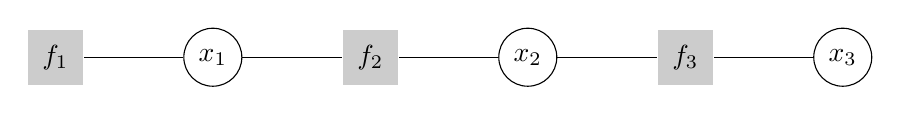
\begin{tikzpicture}
			\tikzset{vertex/.style = {shape=circle,draw,minimum size=1.5em}}
			\tikzset{edge/.style = {-,> = latex'}}
			
			\node[vertex] (x1) at  (0,0) {$x_1$};
			\node[vertex] (x2) at  (4,0) {$x_2$};
			\node[vertex] (x3) at  (8,0) {$x_3$};
			
			\tikzset{vertex/.style = {shape = rectangle,fill = gray!40,minimum size=2em}}
			\node[vertex] (f1) at  (-2,0) {$f_1$};
			\node[vertex] (f2) at  (2,0) {$f_2$};
			\node[vertex] (f3) at  (6,0) {$f_3$};
			
			\draw[edge] (x1) to (f1);
			\draw[edge] (x1) to (f2);
			\draw[edge] (x2) to (f2);
			\draw[edge] (x2) to (f3);
			\draw[edge] (x3) to (f3);
			\end{tikzpicture}
		\end{figure}
	
	\begin{equation*}
	p(X)= \prod_{s} f_s(X_s)
	\end{equation*}}
	\end{frame}
	
\section{Message passing}

\begin{frame}[t]{Message passing: Idea}
	
	\begin{equation*}
	p(X)= \prod_{s} f_s(X_s)
	\end{equation*}
	\begin{figure}
		\centering
		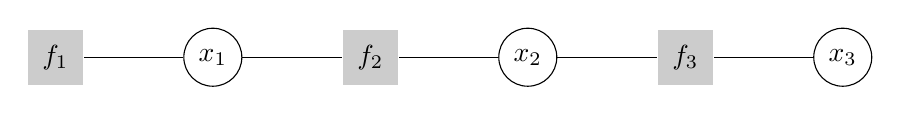
\begin{tikzpicture}
		\tikzset{vertex/.style = {shape=circle,draw,minimum size=1.5em}}
		\tikzset{edge/.style = {-,> = latex'}}
		
		\node[vertex] (x1) at  (0,0) {$x_1$};
		\node[vertex] (x2) at  (4,0) {$x_2$};
		\node[vertex] (x3) at  (8,0) {$x_3$};
		
		\tikzset{vertex/.style = {shape = rectangle,fill = gray!40,minimum size=2em}}
		\node[vertex] (f1) at  (-2,0) {$f_1$};
		\node[vertex] (f2) at  (2,0) {$f_2$};
		\node[vertex] (f3) at  (6,0) {$f_3$};
		
		\draw[edge] (x1) to (f1);
		\draw[edge] (x1) to (f2);
		\draw[edge] (x2) to (f2);
		\draw[edge] (x2) to (f3);
		\draw[edge] (x3) to (f3);
		\end{tikzpicture}
	\end{figure}
	
	\only<2->{Marginalization naive:
	\begin{equation*}
	p(x_2)= \sum_{x_1} \sum_{x_3} p(X) \in \mathcal{O}(k^n)
	\end{equation*}}
	\only<3->{Marginalization advanced:
	\begin{equation*}
	\begin{split}
	p(x_2) &= \sum_{x_1} \sum_{x_3} p(x_1) p(x_2|x_1) p(x_3|x_2) \\ &= \underbrace{\Big[ \sum_{x_1}  p(x_1) p(x_2|x_1)\Big]}_{\mu_{f_2 \rightarrow x_2}}\cdot \underbrace{\Big[ \sum_{x_3}  p(x_3|x_2)\Big]}_{\mu_{f_3 \rightarrow x_2}} \in \mathcal{O}(n \cdot k^2)
	\end{split}
	\end{equation*}}
\end{frame}

\begin{frame}[t]{Sum-product algorithm 1}
	General marginalization:
	\begin{equation*}\label{eq:message1}
	p(x_i) = \prod_{s \in ne(x_i)} \mu_{f_s \rightarrow x_i}(x_i)
	\end{equation*}
	\begin{figure}[h]
		\centering
		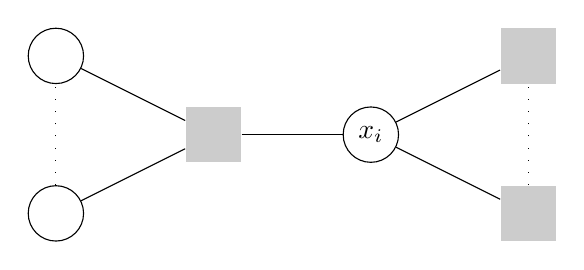
\begin{tikzpicture}
		
		\definecolor{darkgreen}{RGB}{59,136,59}
		
		\tikzstyle{edge} = [draw,-]
		%\fill[green!20]   (0:-1.2) circle (1.8);
		%\node[darkgreen] (text) at (-0.6,1) {$F_s(x_i,X_s)$};
		
		%\fill[green!20]   (4.1,-1.1) circle (0.8);
		%\fill[green!20]   (4.1,1.1) circle (0.8);
		
		\tikzset{vertex/.style = {shape=circle,draw,minimum size=2em}}
		\node[vertex] (xi) at  (2,0) {$x_i$};
		\node[vertex] (xl1) at  (-2,-1) {};
		\node[vertex] (xl2) at  (-2,1) {};
		%\node[vertex] (xrr1) at  (6,-2) {};
		%\node[vertex] (xrr2) at  (6,0) {};
		
		\tikzset{vertex/.style = {shape = rectangle,fill = gray!40,minimum size=2em}}
		\node[vertex] (fs) at  (0,0) {};
		\node[vertex] (xr1) at  (4,-1) {};
		\node[vertex] (xr2) at  (4,1) {};
		%\node[vertex] (xll1) at  (-4,-2) {};
		%\node[vertex] (xll2) at  (-4,0) {};
		
		\draw[edge] (fs) to (xi);
		\draw[edge] (xi) to (xr1);
		\draw[edge] (xi) to (xr2);
		\draw[edge] (fs) to (xl1);
		\draw[edge] (fs) to (xl2);
		%\draw[edge] (xr1) to (xrr1);
		%\draw[edge] (xr1) to (xrr2);
		%\draw[edge] (xl1) to (xll1);
		%\draw[edge] (xl1) to (xll2);
		\draw[edge, loosely dotted] (xr1) to (xr2);
		\draw[edge, loosely dotted] (xl1) to (xl2);
		\end{tikzpicture}
	\end{figure}
\end{frame}

\begin{frame}[t]{Sum-product algorithm 2}
	Local messages through factor graph:
	\begin{equation*}
	\begin{split}
	\mu_{f_s \rightarrow x_i}(x_i) &= \sum_{\mathbf{x_s} \setminus x_i} f_s(x_i, X_s) \prod_{m \in ne(f_s) \setminus x_i} \mu_{x_m \rightarrow f_s}(x_m)\\
	\mu_{x_m \rightarrow f_s}(x_m) &= \prod_{l \in ne(x_m) \setminus f_s} \mu_{f_l \rightarrow x_m}(x_m)
	\end{split}
	\end{equation*}
	
	\begin{figure}[h]
		\centering
		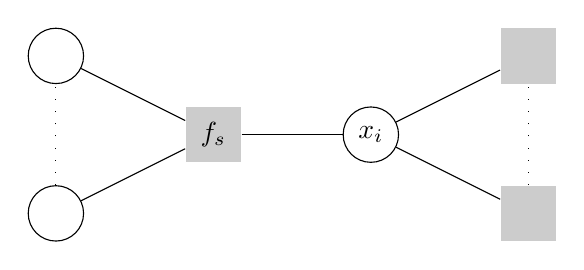
\begin{tikzpicture}
		
		\definecolor{darkgreen}{RGB}{59,136,59}
		
		\tikzstyle{edge} = [draw,-]
		%\fill[green!20]   (0:-1.2) circle (1.8);
		%\node[darkgreen] (text) at (-0.6,1) {$F_s(x_i,X_s)$};
		
		%\fill[green!20]   (4.1,-1.1) circle (0.8);
		%\fill[green!20]   (4.1,1.1) circle (0.8);
		
		\tikzset{vertex/.style = {shape=circle,draw,minimum size=2em}}
		\node[vertex] (xi) at  (2,0) {$x_i$};
		\node[vertex] (xl1) at  (-2,-1) {};
		\node[vertex] (xl2) at  (-2,1) {};
		%\node[vertex] (xrr1) at  (6,-2) {};
		%\node[vertex] (xrr2) at  (6,0) {};
		
		\tikzset{vertex/.style = {shape = rectangle,fill = gray!40,minimum size=2em}}
		\node[vertex] (fs) at  (0,0) {$f_s$};
		\node[vertex] (xr1) at  (4,-1) {};
		\node[vertex] (xr2) at  (4,1) {};
		%\node[vertex] (xll1) at  (-4,-2) {};
		%\node[vertex] (xll2) at  (-4,0) {};
		
		\draw[edge] (fs) to (xi);
		\draw[edge] (xi) to (xr1);
		\draw[edge] (xi) to (xr2);
		\draw[edge] (fs) to (xl1);
		\draw[edge] (fs) to (xl2);
		%\draw[edge] (xr1) to (xrr1);
		%\draw[edge] (xr1) to (xrr2);
		%\draw[edge] (xl1) to (xll1);
		%\draw[edge] (xl1) to (xll2);
		\draw[edge, loosely dotted] (xr1) to (xr2);
		\draw[edge, loosely dotted] (xl1) to (xl2);
		\end{tikzpicture}
	\end{figure}

	\only<2->{Initialization at leaf nodes:
		$\mu_{x \rightarrow f}(x) = 1$, $\mu_{f \rightarrow x}(x) = f(x)$}
\end{frame}

\begin{frame}{Message passing in action}
	\begin{figure}[h]
		\centering
		\begin{tikzpicture}
		
		\definecolor{darkgreen}{RGB}{59,136,59}
		
		\tikzstyle{edge} = [draw,-]
		%\fill[green!20]   (0:-1.2) circle (1.8);
		%\node[darkgreen] (text) at (-0.6,1) {$F_s(x_i,X_s)$};
		
		%\fill[green!20]   (4.1,-1.1) circle (0.8);
		%\fill[green!20]   (4.1,1.1) circle (0.8);
		
		\tikzset{vertex/.style = {shape=circle,draw,minimum size=2em}}
		\node[vertex] (xi) at  (2,0) {$x_i$};
		\node[vertex] (xl1) at  (-2,-1) {};
		\node[vertex] (xl2) at  (-2,1) {};
		\node[vertex] (xrr1) at  (6,-2) {};
		\node[vertex] (xrr2) at  (6,0) {};
		
		\tikzset{vertex/.style = {shape = rectangle,fill = gray!40,minimum size=2em}}
		\node[vertex] (fs) at  (0,0) {};
		\node[vertex] (xr1) at  (4,-1) {};
		\node[vertex] (xr2) at  (4,1) {};
		\node[vertex] (xll1) at  (-4,-2) {};
		\node[vertex] (xll2) at  (-4,0) {};
		
		
		\draw[edge] (xl1) to (xll1);
		\draw[edge] (xl1) to (xll2);
		
		
		\draw[edge] (fs) to (xi);
		\draw[edge] (xi) to (xr1);
		\draw[edge] (xi) to (xr2);
		\draw[edge] (fs) to (xl1);
		\draw[edge] (fs) to (xl2);
		\draw[edge] (xr1) to (xrr1);
		\draw[edge] (xr1) to (xrr2);
		
		
		\only<2-4>{
			\draw[edge, red, <-] (xl1) to (xll1);
			\draw[edge, red, <-] (xl1) to (xll2);
			\draw[edge, red, <-] (xr1) to (xrr1);
			\draw[edge, red, <-] (xr1) to (xrr2);
			\draw[edge, red, <-] (fs) to (xl2);
			\draw[edge, red, <-] (xi) to (xr2);
	}
		
		\only<3-4>{
			\draw[edge, blue, <-] (fs) to (xl1);
			\draw[edge, blue, <-] (xi) to (xr1);
		}
		\only<4-4>{
			\draw[edge, green, <-] (xi) to (fs);
		}
	
		\only<5->{
			\draw[edge, orange, ->] (xi) to (xr2);
			\draw[edge, orange, ->] (xi) to (xr1);
			\draw[edge, orange, ->] (xi) to (fs);
		}
	
		\only<6->{
			\draw[edge, orange, ->] (xr1) to (xrr2);
			\draw[edge, orange, ->] (xr1) to (xrr1);
			\draw[edge, orange, ->] (fs) to (xl1);
			\draw[edge, orange, ->] (fs) to (xl2);
		}
%		\only<7->{
%			\draw[edge, violet, ->] (xl1) to (xll2);
%			\draw[edge, violet, ->] (xl1) to (xll1);
%		}
		%\draw[edge, loosely dotted] (xr1) to (xr2);
		%\draw[edge, loosely dotted] (xl1) to (xl2);
		\end{tikzpicture}
	\end{figure}
\end{frame}

\begin{frame}[t]{Maximum aposteriori estimation}
	\begin{figure}
	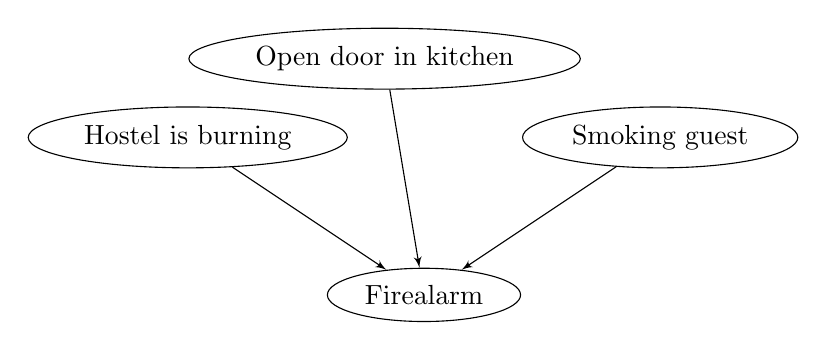
\begin{tikzpicture}
	
	\tikzset{vertex/.style = {shape=ellipse,draw,minimum size=1.5em}}
	\tikzset{edge/.style = {->,> = latex'}}
	
	\node[vertex] (x1) at  (3,-2) {Smoking guest};
	\node[vertex] (x2) at  (-3,-2) {Hostel is burning};
	\node[vertex] (x3) at  (0,-4) {Firealarm};
	\node[vertex] (x4) at  (-0.5,-1) {Open door in kitchen};
	%\node[vertex] (x5) at  (-0.5,1) {Breakfast is prepared};
	
	\draw[edge] (x1) to (x3);
	\draw[edge] (x2) to (x3);
	\draw[edge] (x4) to (x3);
	%\draw[edge] (x5) to (x4);
	\end{tikzpicture}
\end{figure}
	\only<2>{\begin{equation*}\label{eq:map_problem}
	X^* = \underset{X}{\arg\max}~ p(X)
	\end{equation*}}
\end{frame}

\begin{frame}[t]{Max-sum algorithm}
	Maximum aposteriori estimation:
	\begin{equation*}\label{eq:map_problem}
	X^* = \underset{X}{\arg\max}~ p(X) = \underset{X}{\arg\max}~ \ln (p(X))
	\end{equation*}
		\only<2->{Infer $p(X^*)$ by adapting sum-product algorithm:
	\begin{equation*}
	\begin{split}
	\mu_{f_s \rightarrow x_i}(x_i) &= \max_{X_s \setminus x_i} \Big[f_s(x_i, X_s) \sum_{m \in ne(f_s) \setminus x_i} \mu_{x_m \rightarrow f_s}(x_m) \Big]\\
	\mu_{x_m \rightarrow f_s}(x_m) &= \sum_{l \in ne(x_m) \setminus f_s} \mu_{f_l \rightarrow x_m}(x_m)
	\end{split}
	\end{equation*}}
	\only<3->{Initialization at leaf nodes:
	$\mu_{x \rightarrow f}(x) = 0$, $\mu_{f \rightarrow x}(x) = \ln f(x)$\\~\\}
	\only<4->{Keep track of maximal X values!}
\end{frame}

\begin{frame}{Message passing: Discussion}
	\begin{itemize}[<+->]
		\item Linear complexity in the number of involved variables
		\item Only exact for trees
		\item In general graphs: Loopy belief propagation
		\item Linearized message passing
	\end{itemize}
\end{frame}

\section{Expectation propagation}
%\begin{frame}{Motivation for approximate inference}
%	Image de-noising:\\
%	\centering
	%\begin{columns}[c] % the "c" option specifies center vertical alignment
	%		\column{.5\textwidth} 
	%		\only<2->{\includegraphics[scale=0.25]{BN_example.png}}
	%		\column{.5\textwidth} 
%	\includegraphics[scale=0.3]{de-noising.png}\\ 
%	$\mathbf{X}$ true image, $\mathbf{Y}$ noisy observation\\~\\
	%	\end{columns}
	%	
	%	\raggedright
	%	\tiny{\only<2->{Image sources:\\
	%%ttp://www.bayesia.com/hs-fs/hubfs/Bayesian\_Networks/Fig\_2\_2\_Sprinkler.png?t=1495201256220\\\&width=450\&height=626\&name=Fig\_2\_2\_Sprinkler.png\\}
	%	
%	\tiny{Figure taken from Bishop: Pattern Recognition and Machine Learning.}
%\end{frame}


\begin{frame}[t]{Expectation propagation: Methodology}
	Intractable true posterior distribution:
	\begin{equation*}
	p(X|\mathcal{D}) = \frac{1}{Z} \prod_i f_i(X)
	\end{equation*}
	\only<2->{Approximating function from exponential family:
	\begin{equation*}
	q(X) = \frac{1}{Z}\prod_i \tilde{f}_i(X)
	\end{equation*}}
	\only<3->{	Minimize KL divergence:
		\begin{equation*}
		KL(p||q) = \int_X p(X) \ln \frac{p(X)}{q(X)}
		\end{equation*}}
	\centering
	\only<4->{Moment matching!}
\end{frame}

\begin{frame}[t]{Expectation propagation: Minimize KL-divergence}
	Complete function:
	\begin{equation*}
	KL \Big( \prod_{i} f_i(X) \Big| \Big| \prod_i \tilde{f}_i(X) \Big)~~~~\text{\textcolor{red}{intractable}}
	\end{equation*}
	\only<2->{All factors independently:
		\begin{equation*}
		KL \Big(f_i(X) \Big| \Big| \tilde{f}_i(X) \Big)~~~~\text{\textcolor{red}{simple, non-iterative, inaccurate}}
		\end{equation*}}
	\only<3->{
	One factor at a time:
	\begin{equation*}
	KL \Big( \prod_{i} f_i(X) \Big| \Big| f_i(X) \cdot \prod_{j \ne i} \tilde{f}_j(X) \Big)~~~~\text{\textcolor{red}{simple, iterative, accurate}}
	\end{equation*}
	}
\end{frame}

\begin{frame}[t]{Expectation propagation: Algorithm}
	Input: $ \forall i: f_i(X)$\\~\\
	Initialization: $\forall i: \tilde{f}_i(X) = 1$\\~\\
	\only<2->{Iteratively refine one factor at a time until convergence:
		\begin{equation*}
		\begin{split}
		q^{\backslash j}(\theta) &= \prod_{i\ne j} \tilde{f}_i(\theta)\\
		q^{new}(\theta) & \propto f_j ~ q^{\backslash j}(\theta)\\
		\tilde{f}_j &= \frac{1}{Z_j} \frac{q^{new}(\theta)}{q^{\backslash j}(\theta)}
		\end{split}
		\end{equation*}}
	
\end{frame}

\begin{frame}[t]{Expectation propagation: Discussion}
	\begin{itemize}[<+->]
		\item Can be applied to any graphical model
		\item Expectation propagation is not guaranteed to converge
		\item If EP converges, it often outperforms VI
		\item Sum-product algorithm special case of EP with fully factorized approximation function
	\end{itemize}
	\only<5->{\begin{figure}[h]
		\begin{center}
			\includegraphics[scale=0.15]{loppyBPasEP.png}
		\end{center}
	\end{figure}}
\end{frame}

\begin{frame}[t]{EP vs. VI}
	Expectation propagation: Minimize $KL(p||q) = \int p \ln \frac{p}{q}$\\
	~\\
	Variational inference: Minimize $KL(q||p)  = \int q \ln \frac{q}{p}$
	\only<2->{
	\begin{figure}[h]
		\begin{center}
			\includegraphics[scale=0.17]{../multimodal_approximation.png}
		\end{center}
	\end{figure}
	\tiny{Figure taken from Bishop: Pattern Recognition and Machine Learning.}}
\end{frame}

\begin{frame}{}
	\centering
	Thanks for your attention!\\
	Questions?
\end{frame}

\begin{frame}{Loopy BP as special case of EP}
	\begin{figure}[h]
		\begin{center}
			\includegraphics[scale=0.15]{loppyBPasEP.png}
		\end{center}
	\end{figure}
	\begin{itemize}[<+->]
	\item Fully factorized approximation function
	\item Refinement step in EP
	\item If EP converges, it often outperforms VI
\end{itemize}
\end{frame}

\end{document}
